\documentclass[letterpaper,12pt]{article}
\usepackage{array}
\usepackage{threeparttable}
\usepackage{geometry}
\geometry{letterpaper,tmargin=1in,bmargin=1in,lmargin=1.25in,rmargin=1.25in}
\usepackage{fancyhdr,lastpage}
\pagestyle{fancy}
\lhead{}
\chead{}
\rhead{}
\lfoot{\footnotesize\textsl{MACS 30123, Spring 2020, PS\#1}}
\cfoot{}
\rfoot{\footnotesize\textsl{Page \thepage\ of \pageref{LastPage}}}

\usepackage{listings}
\lstset{
   frame=single,
   language=Python,
   showstringspaces=false,
   columns=flexible,
   basicstyle={\small\ttfamily},
   numbers=none,
   breaklines=true,
   breakatwhitespace=true,
   tabsize=4
}

\usepackage{mathtools}
\DeclarePairedDelimiter\abs{\lvert}{\rvert}
\DeclarePairedDelimiter\norm{\lVert}{\rVert}

\renewcommand\headrulewidth{0pt}
\renewcommand\footrulewidth{0pt}
\usepackage[format=hang,font=normalsize,labelfont=bf]{caption}
\usepackage{amsmath}
\usepackage{amssymb}
\usepackage{amsthm}
\usepackage{natbib}
\usepackage{setspace}
\usepackage{float,color}
\usepackage[pdftex]{graphicx}
\usepackage{hyperref}
\hypersetup{colorlinks,linkcolor=red,urlcolor=blue,citecolor=red}
\theoremstyle{definition}
\newtheorem{theorem}{Theorem}
\newtheorem{acknowledgement}[theorem]{Acknowledgement}
\newtheorem{algorithm}[theorem]{Algorithm}
\newtheorem{axiom}[theorem]{Axiom}
\newtheorem{case}[theorem]{Case}
\newtheorem{claim}[theorem]{Claim}
\newtheorem{conclusion}[theorem]{Conclusion}
\newtheorem{condition}[theorem]{Condition}
\newtheorem{conjecture}[theorem]{Conjecture}
\newtheorem{corollary}[theorem]{Corollary}
\newtheorem{criterion}[theorem]{Criterion}
\newtheorem{definition}[theorem]{Definition}
\newtheorem{derivation}{Derivation} % Number derivations on their own
\newtheorem{example}[theorem]{Example}
\newtheorem{exercise}[theorem]{Exercise}
\newtheorem{lemma}[theorem]{Lemma}
\newtheorem{notation}[theorem]{Notation}
\newtheorem{problem}[theorem]{Problem}
\newtheorem{proposition}{Proposition} % Number propositions on their own
\newtheorem{remark}[theorem]{Remark}
\newtheorem{solution}[theorem]{Solution}
\newtheorem{summary}[theorem]{Summary}
%\numberwithin{equation}{section}
\bibliographystyle{aer}
\newcommand\ve{\varepsilon}
\newcommand\boldline{\arrayrulewidth{1pt}\hline}


\begin{document}

\begin{flushleft}
  \textbf{\large{Problem Set \#1}} \\
  MACS 30250, Dr. Clindaniel \\
  Due Wenesday, April 29 at 5:00pm
\end{flushleft}

\vspace{5mm}

\begin{enumerate}
  \item \textbf{Clocking parallelism.} In this exercise, you will document the degree to which a parallel processing approach speeds up the compute time of your entire program as you increase the number of CPU's. Let $z_t$ be an individual's health index value in period $t$, where each period is a week. A high value of $z_t$ signifies good health and a low value of $z_t$ signifies bad health. Assume you are studying the properties of the health of individuals over time $z_t$, which follows an AR(1) process (persistence) and has a normally distributed idiosyncratic error,
  \begin{equation*}
    z_{t} = \rho z_{t-1} + (1-\rho)\mu + \ve_t \quad\text{where}\quad \ve_t\sim N(0,\sigma)
  \end{equation*}
  where $\rho\in[-0.95,0.95]$ represents the degree of persistence in the process, $\mu$ is the long-run average value of the time series, and $\sigma$ is the standard deviation of the normally distributed idiosyncratic errors. Because you don't know what health shocks $\ve_t$ an individual will get, one way to study this is to simulate many lifetimes of health shocks and the resulting outcomes on the individual's health index $z_t$. The following code is how you would simulate 1,000 lifetimes of health shocks, each lifetime being 4,160 weeks (80 years times 52 weeks per year) given the particular parameter values of $\rho=0.5$, $\mu=3$, $\sigma=1$, and $z_0=\mu$.
  \vspace{3mm}
  \begin{lstlisting}
    import numpy as np
    import scipy.stats as sts

    # Set model parameters
    rho = 0.85
    mu = 3.0
    sigma = 0.8
    z_0 = mu

    # Set simulation parameters, draw all idiosyncratic random shocks,
    # and create empty containers
    S = 1000  # Set the number of lives to simulate
    T = int(4160)  # Set the number of periods for each simulation
    np.random.seed(25)
    eps_mat = sts.norm.rvs(loc=0, scale=sigma, size=(T, S))
    z_mat = np.zeros((T, S))
    z_mat[0, :] = z_0

    for s_ind in range(S):
        z_tm1 = z_0
        for t_ind in range(T):
            e_t = eps_mat[t_ind, s_ind]
            z_t = rho * z_tm1 + (1 - rho) * mu + e_t
            z_mat[t_ind, s_ind] = z_t
            z_tm1 = z_t
  \end{lstlisting}
  \vspace{3mm}
  The first 500 periods of the first simulated $z_t$ series in \texttt{z\_mat} is shown in Figure \ref{FigZtPath}. Note that for this particular simulated lifetime, the individual starts at a value below average $z_1<\mu$ and the first period in which her health dips below 0 is $t=8$.

  \begin{figure}[htb]\centering \captionsetup{width=4.5in}
    \caption{\label{FigZtPath}\textbf{Single time path of $z_t$ for first 100 periods}}
    \fbox{\resizebox{4.5in}{3.3in}{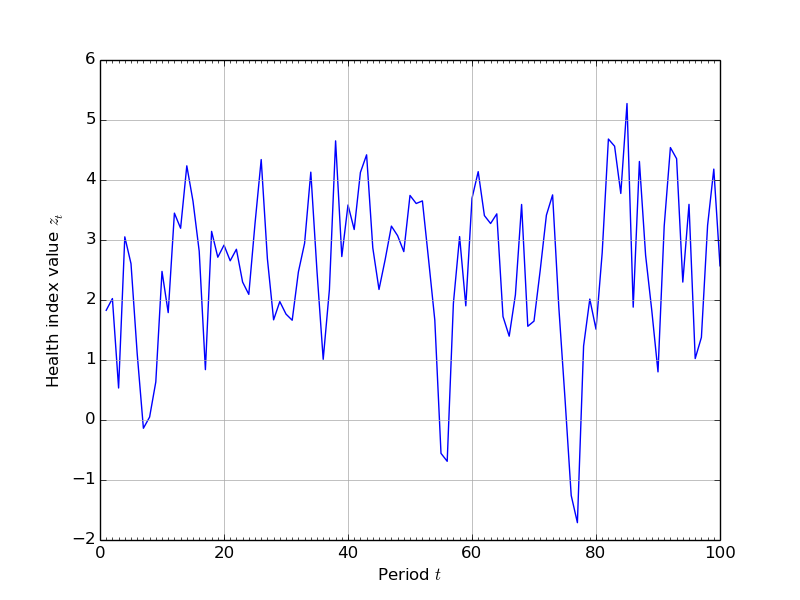
\includegraphics{images/zt_path.png}}}
  \end{figure}

  \begin{enumerate}
    \item Log onto RCC Midway and time 100 different runs of the simulation above---i.e., 100 different runs of 1,000 simulations each of the time series of 4,160 periods. Do one run in serial using only one core as in the code above (1,000 simulations on one core), the second run using two cores (500 simulations per core), the third run using three cores (~333 simulations per core), and the last run using 100 processors (10 simulations per core). Use the \texttt{mpi4py} library to implement your parallelism. Plot the computation time for the 1,000 simulations on the $y$-axis against the number of cores for the particular run on the $x$-axis.
    \item Why is the speedup not linear? That is, why is the 100-core run not 100 times faster than the single-core run?
  \end{enumerate}

  \newpage
  \item \textbf{Embarrassingly parallel processing (grid search).} Assume that really bad things happen to people whose health index falls to or below zero $z_t\leq 0$. And assume that you are concerned about individuals who are already sick or whose current health level is below average $z_0=\mu - 3\sigma$. Assume that you can formulate a health policy that changed the persistence $\rho$ of an individual's health.
  \begin{enumerate}
    \item Use grid search (embarassingly) parallel processing to find the optimal value of $\rho$ that maximizes the number of average number of periods across each of the 1,000 simulations that it takes to first reach a negative health index value $z_t\leq 0$. Perform your grid search over 200 values of $\rho$ equally spaced between -0.95 and 0.95 using the RCC Midway cluster with 100 cores and using \texttt{mpi4py} to implement your parallel processing of two values of $\rho$ per core. Report the computation time to find the optimal $\rho$. [TIPS: Make sure to draw your $T\times S$ matrix of epsilon shocks $\ve_t$ only once at the beginning of this code before any parallel processing is implemented. Then pass that same matrix of shocks into every different value of $\rho$.]
    \item Plot the average periods to the first negative or zero health value $z_t\leq 0$ for each value of $\rho$ (plot $\rho$ values on the $x$-axis and average periods to first negative health value on the $y$-axis.
    \item Report the optimal persistence $\rho$ and the corresponding average periods to negative health.
  \end{enumerate}

  \item \textbf{More sophisticated parallelism (minimizer).} In this exercise, we will perform the same optimization from Exercise 2, but in a more efficient way (should be faster) by embedding the parallel processing inside of a larger serial program. Instead of grid search, we will use a minimizer to find the optimal $\rho$.
  \begin{enumerate}
    \item Use \texttt{scipy.opimize.minimize()} to find the optimal $\rho$. Use an initial guess of $\rho=0.1$. For each guess of $\rho$ that the minimizer makes, use 100 cores on RCC Midway to do the 1,000 simulated time series of $z_t$ (i.e., 10 simulations of the time series per core). Report the computation time to find the optimal $\rho$.
    \item Report the optimal persistence $\rho$ and the corresponding average periods to negative health.
    \item How does the computation time for this Exercise compare to the computation time from Exercise 2? Why is this method faster or slower than the grid search method in Exercise 2?
  \end{enumerate}
\end{enumerate}


% \vspace{25mm}


% \bibliography{PS1.bib}


\end{document}
